\subsection{Encoders}
\label{sec:implementation_encoding}

\begin{figure}[htb]
	\centering
	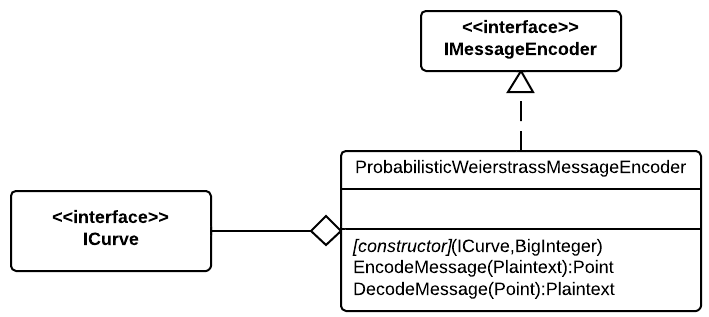
\includegraphics[width=0.7\textwidth]{implementation/encoders}
	\caption{An encoder has a certain amount of state (like the probabilistic encoding's key \(K\), see \ref{sec:math_encoding}), that is
		set in the constructor. The interface requires only an encoding algorithm (\(Plaintext \to Point\)) and
		a decoding algorithm (\(Point \to Plaintext\)).}
\end{figure}

The encoding algorithm introduced in this report, and thus implemented in OpenECC, is probabilistic and supports
only curves in the Weierstrass form. Other algorithms, both supporting other types of curves, and even some being
deterministic, do exist.\cite{MappingAMessage}\cite{InjectiveEncodings}

These other encoding schemes are significantly more mathematically advanced, but they also provide both performance
and probability improvements. Being open for the future addition of these different encoders, and others that may be
discovered, is important for the possible performance of the project.